\chapter{Toolbox}\label{annex:toolbox}

\section{SeapodymView}\label{appendix-toolbox}
The SeapodymView software was designed at SPC to manipulate and visualize DYM files. This software has a dedicated documentation, therefore here we provide only a short description of essential functionalities of SeapodymView that are used more often, recommending to read its reference manual for the complete information. SeapodymView is a java application, which runs both on Linux and Windows. Note, the language settings depend on the computer set-up, so the names in the menus cited here will be different if default language is not English. Several options for the {\ttfamily Look and feel} of the software are available. \\


\subsection{Visualization of DYM variables}

Getting started with SeadpodymView is simple and intuitive. Upon loading, the software opens the dialogue window (Figure~\ref{fig:coloredmap}, panel a) suggesting to select DYM file from the home directory (first load), or from the directory that was previously selected. In the right panel of this dialogue window the software shows the information written in the DYM header. If SeapodymView was already open and one file was already displayed, more files can be loaded from menu {\ttfamily File $\rightarrow$ New}, or by clicking the button {\ttfamily Create a new document}. The software reads the data from selected DYM file and opens the pop-up window displaying its first spatial distribution (Figure~\ref{fig:coloredmap}, panel b).

The map is displayed within the entire latitudinal and longitudinal ranges. It can be zoomed in and out using the mouse wheel. Otherwise the regional zoom can be achieved by selecting the rectangular zone of interest while holding the mouse wheel down. Another click of the mouse wheel on the selected region gets the entire map back. By default, the colorscale for the spatial distribution is confined within the {\ttfamily MIN\_VALUE} and {\ttfamily MAX\_VALUE} written in the DYM file, which is not always optimal in terms of visualization. So, the minimal and maximal displayed values can be modified via right click of the mouth  on the map and selecting {\ttfamily Color palette} from the pop-up menu. Note also that it is possible to see the values on the map with the left mouse click. The value on the intersection of two perpendicular lines are always displayed in the bottom panel of the window, which shows also the current coordinate and the date.

The spatial distributions can be advanced in time with help of buttons on the left-hand panel (green triangles with vertical bar, see Figure~\ref{fig:coloredmap}, panel b). Another useful functionality of SeapodymView is the animation of spatial distributions, controlled with help of buttons {\ttfamily Play the animation}, {\ttfamily Stop the animation} etc. on the left-hand panel. Besides, if several DYM files are displayed, it is possible to synchronize the animation by placing each spatial distribution at the same time step and linking them using button {\ttfamily Select everything}. The speed of animation can be adjusted, see menu {\ttfamily Properties/Advanced}.

Also, SeapodymView can visualize several DYM variables overlayed on the same map. Thus, it is possible to overlay the fish density biomass with other variables, such as sparse catch data, ocean currents, weekly or monthly individual trajectories. See {\ttfamily Properties} in the pop-up menu activated by the right click of the mouse on the map. 

Note that the software allows opening the output DYM file while the simulation is still running. The only condition that is required by SeapodymView is that at least three matrices are written in the DYM file. This functionality can be particularly useful for the long runs, allowing a quick check of the model output without waiting the end of simulation. 


\begin{figure}
\begin{center}
\vbox{
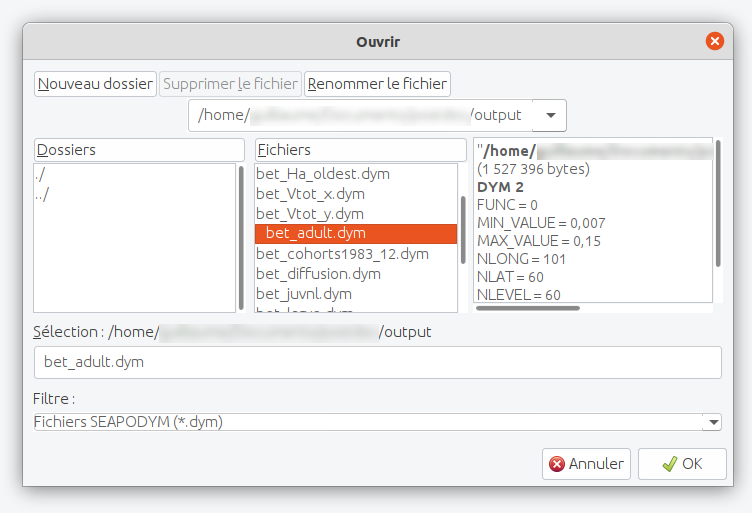
\includegraphics[width=0.9\textwidth,trim=0mm 0mm 0mm 0mm,clip]{annexes/figs/loading_file.png}\\
\vspace{1mm}
(a)\\
}
\vspace{1mm}
\vbox{
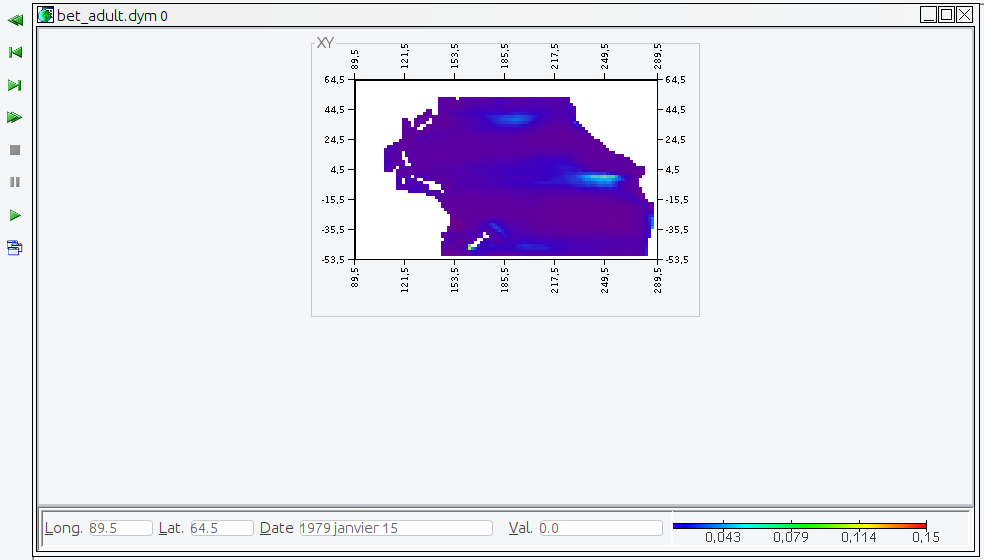
\includegraphics[width=0.9\textwidth,trim=0mm 0mm 0mm 0mm,clip]{annexes/figs/map_loaded.png}\\
\vspace{1mm}
(b) \\
}
\vspace{1mm}
\caption{ Loading a {\bfseries {\ttfamily .dym}} file with Seapodym View. (a) Dialogue window  of the loading file, showing the input directory, the list of DYM files and the contents of the file header. (b) File loaded and map displayed and fully extended on the visualization pane. The colorscale 'Temperature' goes from the dark purple to the red for the lowest to highest values being displayed. The buttons on left-size panel allow playing the animation or to advance the spatial distribution in time by one time step. 
}
\label{fig:coloredmap}
\vspace{-0.0cm}
\end{center}
\end{figure}

\subsection{Temporal and spatial extractions}

SeapodymView can extract DYM variables over the region of interest or over the selected time period (see menu {\ttfamily Tools/Extraction/Seapodym}). Moreover, upon extracting, the variable can be aggregated resulting either in its temporal or spatial average. 

\begin{description}

\item[Temporal averaging => Spatial matrix.] \ 
Let's call $\phi\left(x,y,t\right)$ the value of a DYM variable at the position $\left(x,y\right)$ and at time $t$. A temporal average can be done as $\left(\left<\phi\left(x,y,t\right)\right>_{t}\right)$, where the notation $\left< ... \right>_{i}$ means an average over the dimension $i$. As a result we obtain a two-dimensional distribution of the size derived from the variable's resolution and the selected region.
 
To do that, go to {\ttfamily Tools $\rightarrow$ Extraction $\rightarrow$ Depth averaging}. Then, click on tab {\ttfamily Options} and select {\ttfamily Temporal averaging => Spatial matrix}. Then, go back to the {\ttfamily Selection} tab and adjust the regional coordinates if necessary. Note, the temporal average can either be saved to another DYM ({\ttfamily .dym}) file, or to the ASCII ({\ttfamily .txt}) file. The choice of the file type can be done in the same dialogue window.\\

\item[Spatial averaging => Time series.] \
Here, the following operation is performed with DYM variable: $\phi\left(t\right) = \left<\phi\left(x,y,t\right)\right>_{x,y}$, which provides the temporal evolution of the its average over a given region. So, the result is the time series. 

To do this operation, go to {\ttfamily Tools $\rightarrow$ Extraction $\rightarrow$ Depth averaging}, then in the tab {\ttfamily Options} select {\ttfamily Spatial averaging => Time series}. Go back to the {\ttfamily Selection} tab, and choose the space-time domain to compute average and extract the time series. The output will automatically be saved into an {\ttfamily ASCII} file. \\ 
\end{description}

\subsection{Arithmetic operations}

SeapodymView allows performing basic arithmetic operations with two or more DYM files. To do that, click on  {\ttfamily Tools $\rightarrow$ Math Operation}. The first file has to be selected in the upper panel named {\ttfamily Input file}. Then the user us suggested to choose the {\ttfamily Operator} among implemented addition, subtraction, multiplication, division and power). The variable from selected DYM file can either be multiplied (subtracted...) by the {\ttfamily Coefficient}, or the operation can be performed on several DYM variables. In the latter case, activate the option {\ttfamily Use the sum of these auxiliary files}, and the dialogue window will allow selecting one or several more DYM files. The result of the operation is stored in the new DYM file, its name and location should be specified in the same dialogue before the {\ttfamily Ok} button gets active. Once the prompt message informing on the file creation has popped up, the new file can be loaded and the result of the operation can be viewed.


\subsection{From DYM to ASCII file}

This conversion might be useful to preform quick quantitative analysis or to plot DYM variable or its regional/temporal extractions using high-level programming languages such as \href{https://www.r-project.org/}{\textbf{R}}, \href{https://www.python.org/}{\textbf{Python}}, or \href{https://fr.mathworks.com/?s_tid=gn_logo}{\textbf{Matlab}}. 

To extract the variables into a text file, go to {\ttfamily Tools $\rightarrow$ Extraction $\rightarrow$ Matrix}. Check the path directory. The name will be set automatically depending on the format chosen to store in the matrix. The file {\ttfamily Txt} type is selected automatically. Then in the {\ttfamily Selection} tab choose one of the five variables for extraction. No adjustment is necessary if choosing the spatial coordinates ({\ttfamily XLON},  {\ttfamily YLAT}) or time ({\ttfamily ZLEVEL}) vector. However, when selecting the land mask {\ttfamily Msksp} or the DYM variable ({\ttfamily Data - main data block}), it is possible to specify the region and the time period for extraction. Clicking {\ttfamily Ok} generates the output ASCII file in the selected folder. \\

\section{Grid and Mask Builder}\label{sec:GMB}

To build the grid for the chosen geographic area and to create the multi-layered land mask we suggest to use the software called GMB (Grid and Mask Builder). It allows also manipulation of land mask such as modification of domain boundaries, closure or opening of sea cells, filtering out the small areas (lakes) surrounded by land and so on. Using ETOPO2 (2-minute gridded global relief data, see information on \url{http://www.ngdc.noaa.gov/mgg/global}) topography maps, GMB allows building regular and stretched grids and creating land masks and masks for arbitrary chosen depth level. Note that for the moment we consider regular grids only, i.e., orthogonal grids with constant resolution in latitude and longitude, although the mixed-resolution type grids (e.g. ORCA) might be envisaged for the future releases of the SEAPODYM application with parameter estimation.

GMB was created and further developed as a plugin for SEAPODYM, which accomplishes grid generation, land mask construction and data interpolation on designed grids. For interpolation of input environmental data such as ocean currents, temperature, oxygen and primary production onto new grids, GMB includes a cubic splines interpolation routine and for transferring sparse catch data averaged over square cells there is the routine for redistributing data within new grid cells.

After downloading software create three directories in the folder GMB: {\ttfamily maps, output} and {\ttfamily data}. In order to start working with GMB, you need to have ETOPO2 maps and contour files. If you didn't download them with GMB, you have two options: either extract map directly from NOAA website \href{http://www.ngdc.noaa.gov/mgg/gdas/gd_designagrid.html}{Geodas} or install GEODAS grid translator from \href{http://www.ngdc.noaa.gov/mgg/geodas/geodas.html}. Current version of GMB reads binary files with GRD98 header (extension g98), data should be written in little-endian, 4-byte integer format. All these settings should be chosen while retrieving map interactively from website or from installed GEODAS software.

To run GMB under Windows or Linux, one must have Java Runtime Environment installed (for latest version go to website \href{http://java.sun.com/j2se/1.5.0/download.jsp}). In Windows, click on jar file in order to run the software. If you are going to work with large, high resolution topography maps, it's better to allocate more memory by typing command from the current GMB directory:

\vspace{0.5cm}
{\ttfamily C:\char`\\WINNT\char`\\system32\char`\\java.exe -Xmx512m -jar GMB.jar}
\vspace{0.35cm}

\noindent in Command Prompt window or simply create shortcut for GMB and indicate it in a Target field. For example,

\vspace{0.5cm}
{\ttfamily C:\char`\\WINNT\char`\\system32\char`\\java.exe -Xmx512m -jar "C:\char`\\Seapodym\char`\\GMB\char`\\GMB.jar" }
\vspace{0.35cm}

\noindent If you run GMB under Linux, type in terminal

\vspace{0.5cm}
{\ttfamily java -jar GMB.jar}
\vspace{0.35cm}

\noindent from directory with jar file. Read GMB help (or directly {\ttfamily readme.txt}) for more details on the functionalities implemented in this software. 

\begin{figure}[t]
   \centering
    \vbox{
    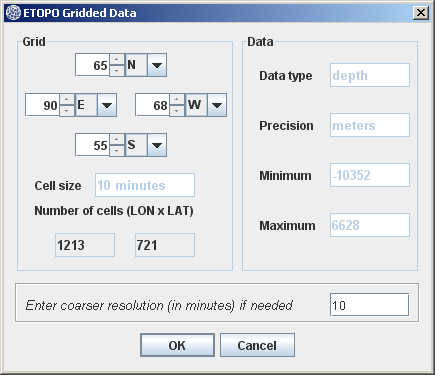
\includegraphics[width=0.7\textwidth]{annexes/figs/GMB-etopo}\\
   }
   \caption{{\bfseries} Loading the map of Pacific Ocean.}
   \label{fig:etopo}
 \end{figure}

For example, to create a $1^{\circ}$ grid for Pacific Ocean domain as shown in Fig~\ref{fig:etopo} and 3-layer mask using GMB, extract the map for the area of interest with ETOPO topographic data (Fig~\ref{fig:etopo}), follow the steps: choose the following menu commands (GMB user's menu activates successively) or click on the corresponding buttons: 1) Load Map; 2) Build Grid; 3) Create Mask; 4) Mask/Apply Boundary Filter. Available Etopo maps with different resolution are stored in the directory {\ttfamily maps}, the files having extension {'\ttfamily .g98}. While extracting geographic area and buiding grid remember that approximation scheme of PDEs in SEAPODYM is based on Arakawa A grid, so first, the domain coordinates must be extended by half of a desired grid resolution, i.e to  {\ttfamily longitudeMin}-$.5\Delta x$, {\ttfamily latitudeMax}-$.5\Delta y$ and so forth; and second, the number of longitudinal and latitudinal grid nodes must be $n_x+1$ and $n_y+1$, where $n_x \times n_y$ is the dimension of all model variables. The decision on the model grid resolution should rely on the following information: 1) the dimension of available physical and biogeochemical variables, either predicted with models (OGCM, NPZD) or observed,  2) the size of the grid cells should be sufficiently small to resolve studied dynamical features, 3) the resolution of available geo-referenced fishing data.

Note that land mask created directly from topography data can be different from the one being used in OGCM or NPZD models, that is why it is recommended to use the data mask (mask, extracted from oceanographic and biogeochemical data) as an initial land mask (use menu {\ttfamily File/Load mask...}). Adding  more layers to the mask, e.g., based on the depth defining epipelagic and mesopelagic layers,  can be done in GMB as well (use menu {\ttfamily Mask/Mask properties...} to set the depth and mask flag, then clicking "`create mask"' will add another layer with specified properties). However, this method will work only in case if depth of the layer is considered to be constant. For the definition of variable layer depths a bit more complex procedure must be undertaken (see below). Since the resulting land mask defines the complex boundary of computational domain, an important step to make before saving the mask file, is to mask existing near-border cells which will cause the biomass leak in the finite-difference approximation scheme of ADR equations. Leak occurs when one computational cell is surrounded by three land cells (or if the ocean cells create one-cell channel), as such layout of grid cells makes it problematic to create reflecting boundary condition. The GMB software filters such boundary cells in one click (menu {\ttfamily Mask/Apply boundary filter...}) . Finally, the mask is saved by GMB into a simple text file with the table of numbers, masking land with 0 and ocean (computational) cells with 1, 2 and 3 etc. according to the number of vertical layers specified for the simulation (see Fig. ~\ref{fig:domain}). \\

\begin{figure}[t]
   \centering
    \vbox{
    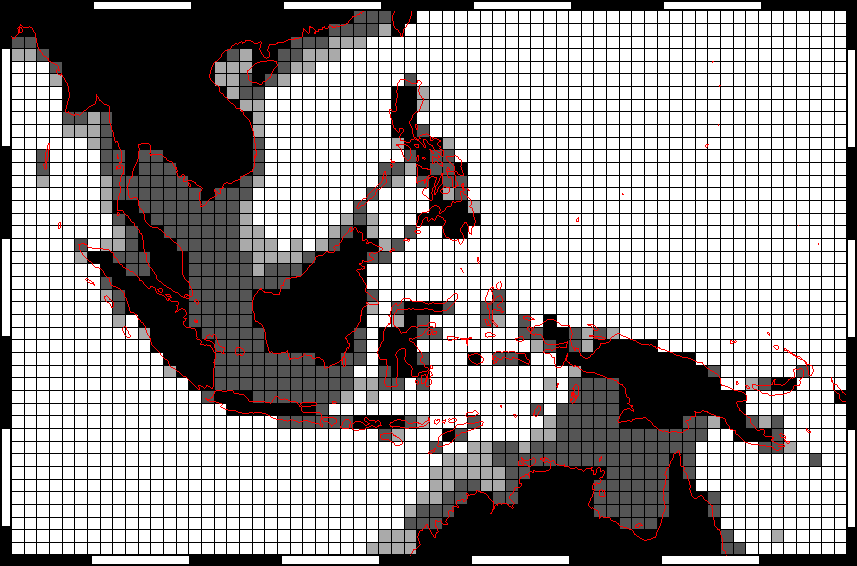
\includegraphics[width=0.75\textwidth]{annexes/figs/Grid-mask}\\
   }
   \caption{{\bfseries} Indo-Pacific regional domain with $1^{\circ}$ grid and 3-layer mask.}
   \label{fig:domain}
 \end{figure}

\section{R scripts}\label{sec:r-tools}

Various R functions were written in order to facilitate data preparation as well as model analyses and validation in SEAPODYM. Here we provide descriptions of only a few selected routines that are essential in extraction of data from SEAPODYM DYM and ASCII files, plotting outputs on a map and preparing fisheries data for simulations with or without scenarios. These functions are part of the following libraries:

\setlength\parindent{2cm}
 
\vspace{0.5cm}
\noindent {\ttfamily dym-works/\\
\indent read\_varDYM.R\\
\indent write\_varDYM.R\\
}

\noindent The example of use of these read-write functions for DYM files \\ 

{\ttfamily  res<-read.var.dym(file.in,t0,tfin,region,deltaT) }\\

\noindent where {\ttfamily t0} and {\ttfamily tfin} are the combinations of two or three values {\ttfamily (year,month,day)}, with {\ttfamily day} which can be omitted for monthly time stepping ({\ttfamily deltaT=30} by default). The returned value of this function, i.e. variable {\ttfamily res} is a {\ttfamily list(x,y,dates,var,landmask)} with the components that are necessary to manipulate DYM data: vectors of coordinates and dates, a variable {\ttfamily var}, extracted over region defined in the corresponding argument and a land mask. There are other useful functions such as {\ttfamily read.txy.dym}  to read only dimensions from a given DYM file, and {\ttfamily read.restart.dym} to read the restart file of SEAPODYM. The syntax for the function to write DYM file is\\

{\ttfamily  write.var.dym(file.out,dates,x,y,landmask,var)}\\

\noindent This function does not return a value, instead the SEAPODYM variable {\ttfamily data.out} is written to a DYM file a {\ttfamily file.out} with all dimensions and a land mask. Another library {\ttfamily fisheries} contains R functions designed to work with SEAPODYM fisheries data files (effort and catch, see ~\ref{sec:EC-datafile}), namely, to read, write fisheries files, compute monthly climatology, introduce effort multipliers, plot final distributions of climatological catch data :\\

\noindent {\ttfamily fisheries/\\
\indent call\_EC\_climatology\_func.R\\
\indent libfd.R\\
\indent make\_EC\_climatology.R\\
\indent rw\_sea\_fisheries.R\\
}\\

\noindent The graphical outputs with fisheries data as well as of extracted DYM variables can be produced with the functions {\ttfamily palettes} and {\ttfamily nice.map} that are implemented in the following files:\\

\noindent {\ttfamily maps/\\
\indent Palette.R\\
\indent plotmaps-GMT.R\\
}\\

\noindent The syntax for {\ttfamily nice.map} function, that will plot the geographical map of the selected region is as follows\\

{\ttfamily  nice.map(x,y,resolution=5,grid=FALSE,...)}\\

\noindent where {\ttfamily x} and {\ttfamily y} are simple increasing values of coordinates, provided as, e.g. {\ttfamily x=100:290, y=-10:10} for tropical Pacific, or {\ttfamily x=-70:20, y=-10:10} for tropical Atlantic. Then, the extracted {\ttfamily var} can be overlaid on the previously plotted map using generic R functions, e.g. {\ttfamily image(x,y,var)}. Note that functions in {\ttfamily plotmaps-GMT.R} use the Generic Mapping Tools (GMT) libraries, therefore before using them check that GMT is installed on your computer. If not, visit page \url{http://gmt.soest.hawaii.edu/projects/gmt/wiki/BuildingGMT} for installation instructions.  \\

\setlength\parindent{1cm}

The installation and the use of these libraries requires two environment variables to be declared in the user's {\ttfamily .bashrc} file:\\

\begin{itemize}
\item[1] {\ttfamily SEA\_R\_HOME}: the path to the folder with all above R scripts
\item[2] {\ttfamily SEA\_HOME}:   the main SEAPODYM directory, with folders called {\ttfamily data} (all forcings placed here), {\ttfamily run} (model runs with parameter files and outputs) and {\ttfamily fisheries} (fisheries data files).
\end{itemize}




